\subsection{Prototyper med fokus på søgefunktionalitet}
\label{subsec:prototype1}

Systemets vigtigste funktionalitet er, at brugerne skal være i stand til at udføre en søgning på nogle råvaretyper, som skal give dem et brugbart resutalt i form af en liste af opskrifter. Uden en søgefunktion er systemet ikke meget værd. Derfor har vi udarbejdet og afprøvet to prototyper, der fokuserer på to forskellige måder, hvorpå man kan udføre en søgning. Den første prototype, som kan ses på \figref{fig:prototype1adesign}, anvendes ved at stave til en råvaretype. Systemet vil ud fra de indtastede bogstaver, give forslag til, hvilke råvaretyper, der er søgbare i systemet. Ud fra den liste, som bliver præsenteret, skal informanten vælge den ønskede råvaretype.

\begin{figure}[H]
	\centering
	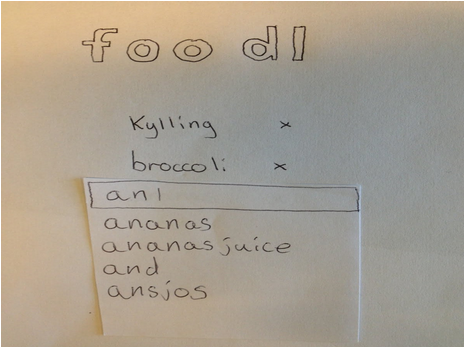
\includegraphics[scale=0.7]{billeder/prototyper/prototype1a.png}
	\capt{Visualisering af prototype 1A, der har fokus på søgefunktionalitet.}
	\label{fig:prototype1adesign}
\end{figure}

På \figref{fig:prototype1adesign} skal det forestille sig, at informanten i forvejen har valgt to råvaretyper (kylling og broccoli). Disse valgte råvaretyper kan fjernes fra søgningen igen ved at klikke på det lille kryds ud for den råvaretype, man vil fjerne. Derudover er informanten i færd med at indtaste et ord, og der er blevet indtastet bogstaverne ``a'' og ``n''. Detmedfører, at systemet giver nogle forslag til søgbare råvaretyper. Man kan vælge at skrive hele ordet færdig eller navigere ned og klikke på den ønskede råvaretype.

Søgefunktionen på \figref{fig:prototype1adesign} minder meget om, hvordan en søgning på \fx Google bliver foretaget. Det er meget minimalistisk, da der et logo og et søgefelt i centrum og dermed i fokus. Google bliver brugt af rigtig mange mennesker\cite{alexaGoogle}. Der er blevet foretaget undersøgelser vedrørende menneskers hukommelse i forhold til genkendelse af objekter og det at skulle komme i tanke om et objekt. Mennesker er meget bedre til at genkende ting, og det er grunden til, at vi prøver at udvikle en søgefunktion, der minder meget om Googles. Der en større chance for, at brugere af systemet kan genkende søgefunktionaliteten og derved være i stand til at udføre en søgning uden problemer, hvis de kan genkende designet \cite[p. ~340]{deb}.

En anden måde, hvorpå en søgefunktion kan designes er præsenteret i \figref{fig:prototype1bdesign}. Her skal man manuelt vælge råvaretyper fra kategoriserede lister. \Fx kan man finde råvaretypen ``kylling'' under kategorien ``Fjerkræ''.

\begin{figure}[H]
	\centering
	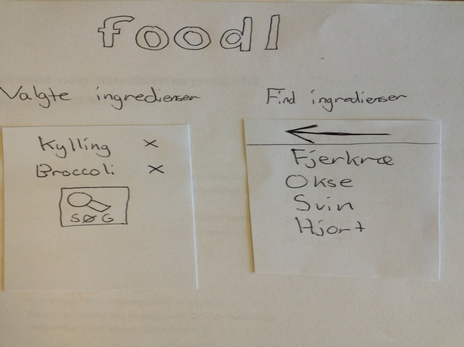
\includegraphics[scale=0.7]{billeder/prototyper/prototype1b.png}
	\capt{Visualisering af prototype 1B, der har fokus på søgefunktionalitet.}
	\label{fig:prototype1bdesign}
\end{figure}

Søgefunktionen på \figref{fig:prototype1bdesign} præsenterer brugeren for to vinduer, hvor man i det venstre vindue kan se, hvilke råvaretyper, man allerede har valgt, og man vælger nye råvaretyper i det højre vindue. Det er i det højre vindue, hvor man skal navigeres sig igennem kategorierne og finde den ønskede råvaretype. Når man har tilføjet alle de ønskede råvaretyper, så kan man udføre en søgning ved at klikke på knappen ``Søg'', som er placeret i det venstre vindue lige under de allerede valgte råvaretyper.

Begge informanter var enige om, at prototypen 1A virkede mere intuitiv og mindre rodet end prototype 1B. Informanterne mente begge, at prototype 1B var langsommere at bruge, og de syntes ikke om den, fordi den faktisk var svær at navigere rundt i. Som et eksempel på, at prototype 1B ikke var intuitiv, er at Merete var i tvivl om, hvilken kategori hun skulle vælge kylling fra (kød eller fjerkræ?). 

Kategorierne kan laves på mange forskellige måder, og uanset hvordan de vælges, vil der med garanti være nogle brugere, der vil være i tvivl om, hvor de skal lede efter en bestemt råvaretype. Begge informanter var enige om, at prototype 1A var hurtig, nem og effektiv at bruge.

På baggrund af informanternes feedback, valgte vi at arbejde videre med prototype 1A. I \secref{sec:webapplikationen} introducerer vi brugergrænsefladen for systemet, hvilket bærer meget præg af vores test med informanterne og disse prototyper.
